\begin{Slide}{Requirements Selection Quality}

Requirements Selection means deciding which features to release.
\begin{itemize}
\item What is a good selection decision?

\item \textbf{If} we had perfect information about all requirements \textbf{and} the ability to precisely predict the future \textbf{then} we could partition all requirements based on their quality (value versus cost):
\begin{itemize}
\item \textbf{Alfa}-requirements: should be \textit{selected} with perfect wisdom
\item \textbf{Beta}-requirements: should be \textit{rejected} with perfect wisdom
\end{itemize}
\end{itemize}
\begin{center}
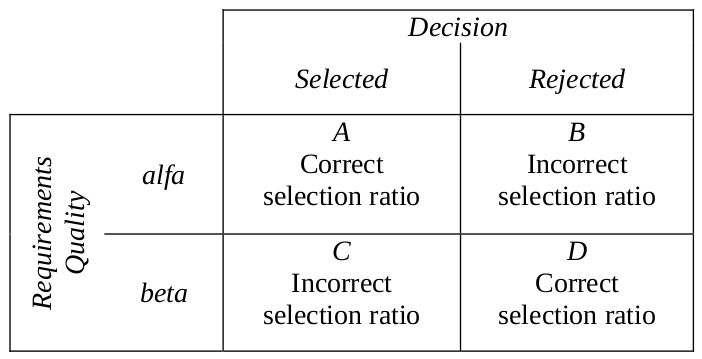
\includegraphics[width=0.6\textwidth]{../img/alfa-beta-reqts}
\end{center}
{
Product quality: \hspace{0.5em}{\Large $\frac{A}{A + C}$}\hfill
Selection quality:\hspace{0.5em}{\Large $\frac{A + D}{A + B + C + D}$}
}

\end{Slide}
